\documentclass{article}

\usepackage[a4paper,margin=2.5cm]{geometry}
\usepackage{tikz}
\usepackage{amsmath}
\usepackage{amssymb}
\usepackage{fancyhdr}
\usepackage{hyperref}
\usepackage{float}
\usepackage{subcaption}
\usepackage{forest}
\usepackage{xcolor}
\usepackage{multirow}
\usepackage{booktabs}
\usepackage{soul}
\usepackage[shortlabels]{enumitem}

\newcommand{\tE}[1]{$\mathbb{E}(\mbox{#1})$}
\newcommand{\E}[1]{\mathbb{E}(\mbox{#1})}
\forestset{
    myedge/.style={if n=1{edge label={node[above left, midway, font=\scriptsize]{#1}}}
                         {edge label={node[above right, midway, font=\scriptsize]{#1}}}}
}
\forestset{
    myarrow/.style={if n=1{edge={->, magenta, line width=1.5pt}, edge label={node[above left, midway, font=\scriptsize]{#1}}}
                          {edge={->, magenta, line width=1.5pt}, edge label={node[above right, midway, font=\scriptsize]{#1}}}}
}

\title{\vspace{-2cm}ECON20005 Assignment 2}
\date{\today}
\author{Lucas Fern (1080613)\\Friday 12:00pm Tutorial}

\lhead{ECON20005 - Assignment 2}
\rhead{Lucas Fern (1080613)}
\pagestyle{fancy}

\begin{document}
\maketitle
\section*{Question 1: Batman or Superman}
\subsection*{1.1}
The normal form of the Friday simultaneous game is:
\begin{table}[H]
    \centering
    \begin{tabular}{@{}cccc@{}}
                                                 &                               & \multicolumn{2}{c}{Lois}                                    \\ \cmidrule(l){3-4} 
                                                 & \multicolumn{1}{c|}{}         & \multicolumn{1}{c|}{Batman} & \multicolumn{1}{c|}{Superman} \\ \cmidrule(l){2-4} 
    \multicolumn{1}{c|}{\multirow{2}{*}{Rachel}} & \multicolumn{1}{c|}{Batman}   & \multicolumn{1}{c|}{\hl{80}, \hl{40}} & \multicolumn{1}{c|}{20, 20}   \\ \cmidrule(l){2-4} 
    \multicolumn{1}{c|}{}                        & \multicolumn{1}{c|}{Superman} & \multicolumn{1}{c|}{20, 20} & \multicolumn{1}{c|}{\hl{30}, \hl{100}}  \\ \cmidrule(l){2-4} 
    \end{tabular}
\end{table}
\noindent Using best response analysis (as shown in the normal form game) the Pure Strategy Nash Equilibria can be found. These are:
\begin{itemize}
    \item (Rachel, Lois) = (Batman, Batman), with equilibrium path Batman $\longrightarrow$ Batman, and payoff $(80, 40)$; and,
    \item (Rachel, Lois) = (Superman, Superman), with equilibrium path Superman $\longrightarrow$ Superman, and payoff $(30, 100)$.
\end{itemize}
To find the mixed strategy NE, define $p$ and $q$ as the probability that Rachel and Lois pick Batman respectively. Starting with Rachel:
\begin{alignat}{3}
    \E{Batman} &= 80q + 20(1-q) &&= 60q + 20\\
    \E{Superman} &= 20q + 30(1-q) &&= 30 - 10q
\end{alignat}
Setting \tE{Batman} $<$ \tE{Superman}:
\begin{align*}
    60q + 20 &< 30 - 10q\\
    70q &< 10\\
    q &< \frac{1}{7}\\
    \implies \E{Batman} &< \E{Superman} \mbox{ for } q < \frac{1}{7}\\
    \implies \E{Batman} &= \E{Superman} \mbox{ for } q = \frac{1}{7}\\
    \implies \E{Batman} &> \E{Superman} \mbox{ for } q > \frac{1}{7}
\end{align*}
Then for Lois:
\begin{alignat}{3}
    \E{Batman} &= 40p + 20(1-p) &&= 20p + 20\\
    \E{Superman} &= 20p + 100(1-p) &&= 100 - 80p
\end{alignat}
Setting \tE{Batman} $<$ \tE{Superman}:
\begin{align*}
    20p + 20 &< 100 - 80p\\
    100p &< 80\\
    p &< \frac{4}{5}\\
    \implies \E{Batman} &< \E{Superman} \mbox{ for } p < \frac{4}{5}\\
    \implies \E{Batman} &= \E{Superman} \mbox{ for } p = \frac{4}{5}\\
    \implies \E{Batman} &> \E{Superman} \mbox{ for } p > \frac{4}{5}
\end{align*}
Since both players are indifferent between the movies at $(p, q) = (\frac{4}{5}, \frac{1}{7})$. This is the mixed strategy Nash equilibrium.

\subsection*{1.2}
The extensive form of the game is:
\begin{figure}[H]
    \centering
    \begin{forest}
        for tree={l=50pt, s sep = 30pt, inner sep=5pt, calign=center}
        [Lois, s sep = 100pt
            [{(45, 85)}, myedge={Don't Buy Tickets}]
            [Rachel, myarrow={Buy Tickets}
                [Lois, myedge=Batman, name=loisl
                    [{(40, 80)}, myedge=Batman]
                    [{(20, 20)}, myarrow=Superman]
                ]
                [Lois, myarrow=Superman, name=loisr
                    [{(20, 20)}, myedge=Batman]
                    [{(100, 30)}, myarrow=Superman]
                ]
            ]
        ]
        \draw[dashed] (loisl) to[out=0,in=180] (loisr);
    \end{forest}
\end{figure}
\noindent The pure strategy Nash equilibrium strategies are shown on the tree as {\color{magenta}pink} arrows. These are 
\begin{itemize}
    \item Lois: (Buy Tickets, Superman) [note that the superman choice applies to both final subgames],
    \item Rachel: Superman.
\end{itemize}
The SPNE path in this case is Buy $\rightarrow$ Superman $\rightarrow$ Superman, and the payoff is $\mbox{(Lois, Rachel)} = (100, 30)$.

\subsection*{1.3}
If the game on Friday is played, Lois' expected payoff is
\begin{align*}
    q \cdot \E{Batman} + (1-q) \cdot \E{Superman} &= \frac{1}{7}(20 \times \frac{4}{5} + 20) + \frac{6}{7}(100 - 80 \times \frac{4}{5})\\
    &= 36
\end{align*}
Since $36 < 45$ Lois will choose to not buy the tickets in this situation, so the SPNE strategies are
\begin{itemize}
    \item Lois: (Don't Buy Tickets, $q = \frac{1}{7}$),
    \item Rachel: $p = \frac{4}{5}$.
\end{itemize}
The SPNE path is `Don't Buy Tickets', which results in a payoff of $\mbox{(Lois, Rachel)} = (45, 85)$.

\subsection*{1.4}
Lois will be indifferent between purchasing and not purchasing tickets as long as her payoff for each option is equal. Her payoff for not purchasing tickets is 45, and her payoff for purchasing them is $105-ticket\ price$, which comes from the outcome where both players watch Superman.\\[2mm]
$105-ticket\ price = 45$ at $ticket\ price = 60$, so at a price of 60 Lois is indifferent between purchasing and not purchasing the tickets.

\section*{Question 2: A pollution game with Australia and New Zealand}
\subsection*{2.1}
The normal form of the game is:
\begin{table}[H]
    \centering
    \begin{tabular}{@{}cccc@{}}
                                             &                         & \multicolumn{2}{c}{NZ}                                  \\ \cmidrule(l){3-4} 
                                             & \multicolumn{1}{c|}{}   & \multicolumn{1}{c|}{NP}    & \multicolumn{1}{c|}{P}     \\ \cmidrule(l){2-4} 
    \multicolumn{1}{c|}{\multirow{2}{*}{AU}} & \multicolumn{1}{c|}{NP} & \multicolumn{1}{c|}{5, 5}  & \multicolumn{1}{c|}{2, \hl{10}} \\ \cmidrule(l){2-4} 
    \multicolumn{1}{c|}{}                    & \multicolumn{1}{c|}{P}  & \multicolumn{1}{c|}{\hl{12}, 1} & \multicolumn{1}{c|}{\hl{3}, \hl{3}}  \\ \cmidrule(l){2-4} 
    \end{tabular}
\end{table}
\noindent The best response analysis as shown in the table gives (AU, NZ) = (P, P) as the only pure strategy Nash equilibrium, this is because NP is a strictly dominated strategy for both players.

\subsection*{2.2}
In the final (50th) subgame it is clear that the NE is (AU, NZ) = (P, P) since the final game is equivalent to the situation where the game is played once. Since the payoff for this outcome is $(3, 3)$, this payoff can be added to the payoffs of the 49th game, giving the following normal form game:
\begin{table}[H]
    \centering
    \begin{tabular}{@{}cccc@{}}
                                             &                         & \multicolumn{2}{c}{NZ}                                  \\ \cmidrule(l){3-4} 
                                             & \multicolumn{1}{c|}{}   & \multicolumn{1}{c|}{NP}    & \multicolumn{1}{c|}{P}     \\ \cmidrule(l){2-4} 
    \multicolumn{1}{c|}{\multirow{2}{*}{AU}} & \multicolumn{1}{c|}{NP} & \multicolumn{1}{c|}{5 + 3, 5 + 3}  & \multicolumn{1}{c|}{2 + 3, \hl{10 + 3}} \\ \cmidrule(l){2-4} 
    \multicolumn{1}{c|}{}                    & \multicolumn{1}{c|}{P}  & \multicolumn{1}{c|}{\hl{12 + 3}, 1 + 3} & \multicolumn{1}{c|}{\hl{3 + 3}, \hl{3 + 3}}  \\ \cmidrule(l){2-4} 
    \end{tabular}
\end{table}
\noindent In this subgame it is clear that (AU, NZ) = (P, P) is still the only Nash equilibrium.\\[2mm]
This logic can be repeated all the way back to the first subgame, with both players choosing P in each of the 50 repetitions of the game.

\subsection*{2.3}
If the countries have agreed to cooperate and both play NP, both their payoffs for the infinitely repeated game are:
$$\sum_{t=0}^{\infty} \delta^{t} \times 5 = \frac{5}{1 - \delta}$$
Australia's payoff for deviating from this strategy and choosing P is:
\begin{align*}
    12 + \sum_{t=1}^{\infty} \delta^{t} \times 3 &= 12 - 3 + \sum_{t=0}^{\infty} \delta^{t} \times 3\\
    &= 9 + \frac{3}{1 - \delta}
\end{align*}
since deviating results in a one-time increased payoff of 12, then infinite payoffs of 3 in future games.\\[2mm]
Similarly, New Zealand's payoff for deviating is
$$10 - 3 + \sum_{t=0}^{\infty} \delta^{t} \times 3 = 7 + \frac{3}{1 - \delta}.$$
In order to cooperate in all periods, the payoff for eternal cooperation must be equal to or greater than the payoff to deviate for both countries. This means that:
\begin{align}
    \frac{5}{1 - \delta} &\geq \mbox{max}\left\{ 9 + \frac{3}{1 - \delta}, 7 + \frac{3}{1 - \delta} \right\}\\
    &\geq 9 + \frac{3}{1 - \delta}\\
    5 &\geq 9(1 - \delta) + 3\\
    9 \delta &\geq 7\\
    \delta &\geq \frac{7}{9}
\end{align}
Therefore $\bar{\delta} = \frac{7}{9}$, since for any lower $\delta$ Australia would receive a higher payoff for deviating.

\subsection*{2.4}
Australia determines the critical value of $\delta$ because they receive a higher one-off payoff for deviating from the cooperative strategy than New Zealand does. This means that Australia will be willing to deviate at a higher discount rate than New Zealand since although they receive an equal payoff for every period in the future, Australia will be able to claim a greater short term advantage.\\[2mm]
This is shown in equation (5)-(6) of the previous question, where Australia's payoff is selected out of the maximum function.

\section*{Question 3: Woolworths-Coles Merger Evaluation by the ACCC}
\subsection*{3.1}
Under Cournot oligopoly the market supply is $Q = q_{W} + q_{C}$, and the inverse demand function can be rewritten as $P(q_{W}, q_{C}) = 100 - 10q_{W} - 10q_{C}$. Woolworths profits in this arrangement are 
$$\Pi_{W} = P(q_{W}, q_{C}) \times q_{W} - c q_{W} = q_{W} \cdot (100 - 10q_{W} - 10q_{C}) - 40 q_{W}$$
and the profit maximising condition for $q_{W}$ is
\begin{align*}
    \frac{\partial \Pi_{W}}{\partial q_{W}} &= 60 - 20 q_{W} - 10 q_{C} = 0\\
    \implies q_{W} &= \frac{6 - q_{C}}{2}.
\end{align*}
By symmetry it is clear that $q_{C} = \frac{6 - q_{W}}{2}$.\\[2mm]
Substituting $q_{C} = \frac{6 - q_{W}}{2}$ into the equation for $q_{W}$:
\begin{align*}
    q_{W} &= \frac{6 - q_{C}}{2}\\
    &= \frac{6 - \frac{6 - q_{W}}{2}}{2}\\
    &= \frac{6 + q_{W}}{4}\\
    4 q_{W} &= 6 + q_{W}\\
    q_{W} &= 2.
\end{align*}
Again by symmetry it is clear that the profit maximising quantity for both firms is $q_{W} = q_{C} = 2$. So:
\begin{itemize}
    \item The equilibrium price is $P(2, 2) = 100 - 20 - 20 = 60$.
    \item The total quantity under Cournot competition is $2 + 2 = 4$.
    \item The consumer surplus is $\int_{Q=0}^{4} P(Q) - \int_{Q=0}^{4} 60 = 320 - 240 = 80$.
    \item The producer surplus is $\int_{Q=0}^{4} 60 - \int_{Q=0}^{4} 40 = 240 - 160 = 80$.
    \item The total surplus is $80 + 80 = 160$.
    \item The socially optimal quantity is $100-10Q = 40 \implies Q = 6$.
    \item Therefore the deadweight loss is $\int_{Q=4}^{6} P(Q) - \int_{Q=4}^{6} 40 = 100 - 80 = 20$.
\end{itemize}

\subsection*{3.2}
Under the merger Wool-Coles is a monopoly, since they observe the same market price $$P(Q) = 100 - 10Q \iff Q(P) = \frac{100 - P}{10}.$$
This means their profit is $\Pi(P) = (P - \tilde{c}) \times \frac{100 - P}{10} = (P - 10) \times \frac{100 - P}{10}$. Finding the profit maximising price:
\begin{align*}
    \frac{\partial \Pi(P)}{\partial P} &= \frac{100 - P}{10} + \frac{-1}{10} (P - 10) = 0\\
    &= 10 - \frac{P}{10} - \frac{P}{10} + 1\\
    \implies P &= 55
\end{align*}
$Q(55) = \frac{100 - 55}{10} = 4.5$ so:
\begin{itemize}
    \item The total quantity under monopoly is $4.5$.
    \item The equilibrium price is $P(4.5) = 55$.
    \item The consumer surplus is $\int_{Q=0}^{4.5} P(Q) - \int_{Q=0}^{4.5} 55 = 348.75 - 247.5 = 101.25$.
    \item The producer surplus is $\int_{Q=0}^{4.5} 55 - \int_{Q=0}^{4.5} 10 = 247.5 - 45 = 202.5$.
    \item The total surplus is $101.25 + 202.5 = 303.75$.
    \item The socially optimal quantity is now $100-10Q = 10 \implies Q = 9$.
    \item Therefore the deadweight loss is $\int_{Q=4.5}^{9} P(Q) - \int_{Q=4.5}^{9} 10 = 146.25 - 45 = 101.25$.
\end{itemize}

\subsection*{3.3}
\begin{figure}[H]
    \centering
    \begin{subfigure}[b]{0.4\linewidth}
      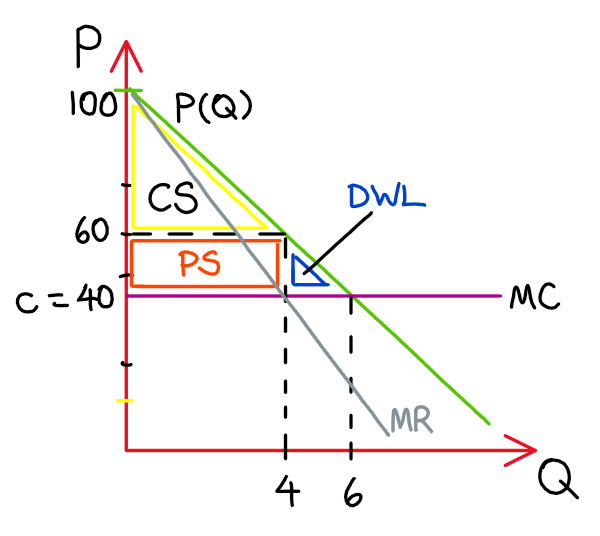
\includegraphics[width=\linewidth]{3-3i.png}
      \caption{A model under Cournot competition.}
    \end{subfigure}
    \begin{subfigure}[b]{0.4\linewidth}
      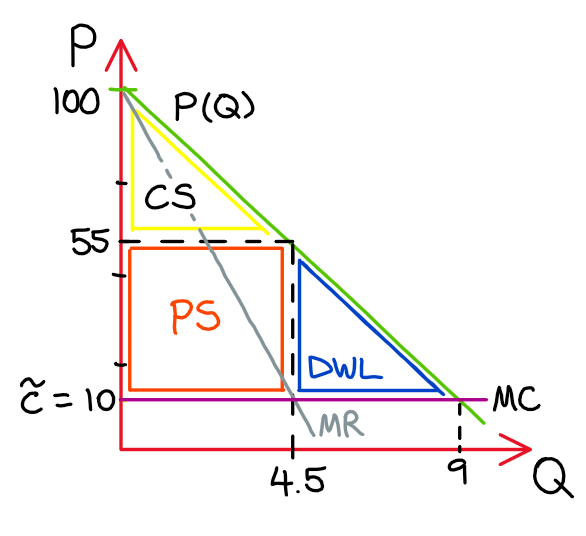
\includegraphics[width=\linewidth]{3-3ii.png}
      \caption{A model under the merger monopoly.}
    \end{subfigure}
    \caption{Sketches of Inverse demand and the market outcome under Oligopoly and Monopoly.}
    \label{fig:Q3.3}
\end{figure}

\subsection*{3.4}
The consumer surplus under Cournot competition is 80. If the merger is approved then the consumer surplus will increase to 101.25. Therefore the ACCC will approve the merger if their goal is to maximise consumer surplus.

\subsection*{3.5}
The total market surplus under Cournot competition is 160. If the merger is approved then the total surplus will increase to 303.75. Therefore the ACCC will approve the merger if their goal is to maximise total market surplus.

\subsection*{3.6}
Writing the profit in terms of $\tilde{c}$ gives $\Pi(P) = (P - \tilde{c}) \frac{100 - P}{10}$. To find the profit maximising quantity in terms of $\tilde{c}$ set the partial derivative equal to zero.
\begin{align*}
    \frac{\partial \Pi(P)}{\partial P} = \frac{100 - P}{10} - \frac{1}{10} (P - \tilde{c}) &= 0\\
    10 - \frac{P}{10} - \frac{P}{10} + \frac{\tilde{c}}{10} &= 0\\
    10 + \frac{\tilde{c}}{10} &= \frac{P}{5}\\
    P &= 50 + \frac{\tilde{c}}{2}
\end{align*}
Then to find the profit maximising quantity in terms of $\tilde{c}$, substitute the formula for maximum profit:
\begin{align*}
    Q(P) &= Q \left( 50 + \frac{\tilde{c}}{2} \right)\\
    &= \frac{100 - (50 + \tilde{c}/2)}{10}\\
    &= \frac{200-100-\tilde{c}}{20}\\
    Q &= \frac{100 - \tilde{c}}{20}
\end{align*}
The consumer surplus is the area bounded by the axis, price, and demand function. Since the demand function is linear in this example, this can be calculated as the area of a triangle. Letting $CS$ be the consumer surplus:
\begin{align*}
    CS &= \frac{(100 - P) \times Q}{2} \mid P \in [0, 100], Q \geq 0\\
    &= \frac{(100 - (50 + \tilde{c} / 2)) \left( \frac{100 - \tilde{c}}{20} \right) }{2}\\
    &= \frac{\left( \frac{100 - \tilde{c}}{2} \right) \left( \frac{100 - \tilde{c}}{20} \right) }{2}\\
    &= \frac{(100 - \tilde{c})^{2}}{80}
\end{align*}
The consumer surplus under Cournot competition was 80, so setting this surplus equal to 80 allows the equation to be solved for the value of $\tilde{c}$:
\begin{align*}
    80 &= \frac{(100 - \tilde{c})^{2}}{80}\\
    \pm \sqrt{6400} &= 100 - \tilde{c}\\
    \tilde{c} &= 100 \pm 80
\end{align*}
Since $\tilde{c} \in [0, 100]$, $\tilde{c} = 100 - 80 = 20$ is the value of $\tilde{c}$ that makes the ACCC indifferent between approving and not approving the merger if its goal is to maximise consumer surplus.

\section*{Question 4: Julia, Kevin, and the Federal Election}
\subsection*{4.1)}
Gillard's payoff is equal to the probability that she wins the election minus the rent-seeking effort $r_{g}$.
$$\Pi_{g} = p_{g} - r_{g} = \frac{0.5 r_{g}}{r_{g} + r_{a}} - r_{g}$$
To maximise this with respect to $r_{g}$, set the partial derivative equal to zero:
\begin{align*}
    \frac{\partial \Pi_{g}}{\partial r_{g}} &= (0.5)\frac{1}{r_{g} + r_{a}} + (0.5 r_{g})\frac{-1}{(r_{g} + r_{a})^2} - 1 = 0\\
    &= \frac{(0.5)r_{a}}{(r_{g} + r_{a})^{2}} - 1\\
    \implies (r_{g} + r_{a})^{2} &= (0.5)r_{a}\\
    r_{g}^2 + 2r_{g}r_{a} + r_{a}^2 &= (0.5)r_{a}\\
    0 &= r_{g}^2 + 2r_{a}r_{g} + (r_{a}^2 - (0.5)r_{a})\\
    \mbox{Solving using the quadratic formula:}\\
    r_{g} &= \frac{-2 r_{a} \pm \sqrt{4 r_{a}^{2} - 4(r_{a}^2 - (0.5)r_{a})}}{2}\\
    &= \frac{-2 r_{a} \pm \sqrt{2 r_{a}}}{2}\\
    &= -r_{a} \pm \sqrt{\frac{r_{a}}{2}}
\end{align*}
Since $r_{g} \geq 0$, $r_{g}^{*} = -r_{a} + \sqrt{{r_{a}}/{2}}$ for $r_{a} \in [0, 0.5]$.

\subsection*{4.2)}
Rudd's payoff is equal to the probability that he wins the election minus the rent-seeking effort $r_{r}$.
$$\Pi_{r} = p_{r} - r_{r} = \frac{0.75 r_{r}}{r_{r} + r_{a}} - r_{r}$$
Maximising again with the partial derivative:
\begin{align*}
    \frac{\partial \Pi_{r}}{\partial r_{r}} &= (0.75)\frac{1}{r_{r} + r_{a}} + (0.75 r_{r})\frac{-1}{(r_{r} + r_{a})^2} - 1 = 0\\
    &\dots\\
    0 &= r_{r}^2 + 2r_{a}r_{r} + (r_{a}^2 - (0.75)r_{a})\\
    \mbox{Solving using the quadratic formula:}\\
    r_{r} &= \frac{-2 r_{a} \pm \sqrt{4 r_{a}^{2} - 4(r_{a}^2 - (0.75)r_{a})}}{2}\\
    &= \frac{-2 r_{a} \pm \sqrt{4 r_{a}^{2} - 4(r_{a}^2 - (0.75)r_{a})}}{2}\\
    &= -r_{a} \pm \frac{\sqrt{3 r_{a}}}{2}\\
    &= -r_{a} \pm \sqrt{\frac{3 r_{a}}{4}}
\end{align*}
Again since $r_{r} \geq 0$, $r_{r}^{*} = -r_{a} + \sqrt{{3 r_{a}}/{4}}$ for $r_{a} \in [0, 0.75]$.

\subsection*{4.3)}
Gillard's optimal rent-seeking effort is:
$$r_{g}^{*}(0.25) = -0.25 + \sqrt{\frac{0.25}{2}} \approx 0.1036$$
And Rudd's is:
$$r_{r}^{*}(0.25) = -0.25 + \sqrt{\frac{3 \times 0.25}{4}} \approx 0.1830$$

\subsection*{4.4)}
To find the probability of each member winning the election, substitute their maximising value of $r$ into their expression for $p$:
\begin{itemize}
    \item Gillard: $$p_{g} = \frac{0.5r_{g}}{r_{g} + r_{a}} = \frac{0.5(-r_{a} + \sqrt{{r_{a}}/{2}})}{r_{a} + (-r_{a} + \sqrt{{r_{a}}/{2}})} = \frac{1}{2} \left( 1 - \sqrt{2 r_{a}} \right)$$
    \item Rudd: $$p_{r} = \frac{0.75r_{r}}{r_{r} + r_{a}} = \frac{0.75(-r_{a} + \sqrt{{3r_{a}}/{4}})}{r_{a} + (-r_{a} + \sqrt{{3r_{a}}/{4}})} = \frac{3}{4} \left( 1 - \sqrt{\frac{4}{3} r_{a}} \right)$$
\end{itemize}
Plotting these probabilities makes it clear that Rudd's probability of winning is greater than Gillard's at all values of $r_{a}$ for which the probability is defined.
\begin{figure}[H]
    \centering
    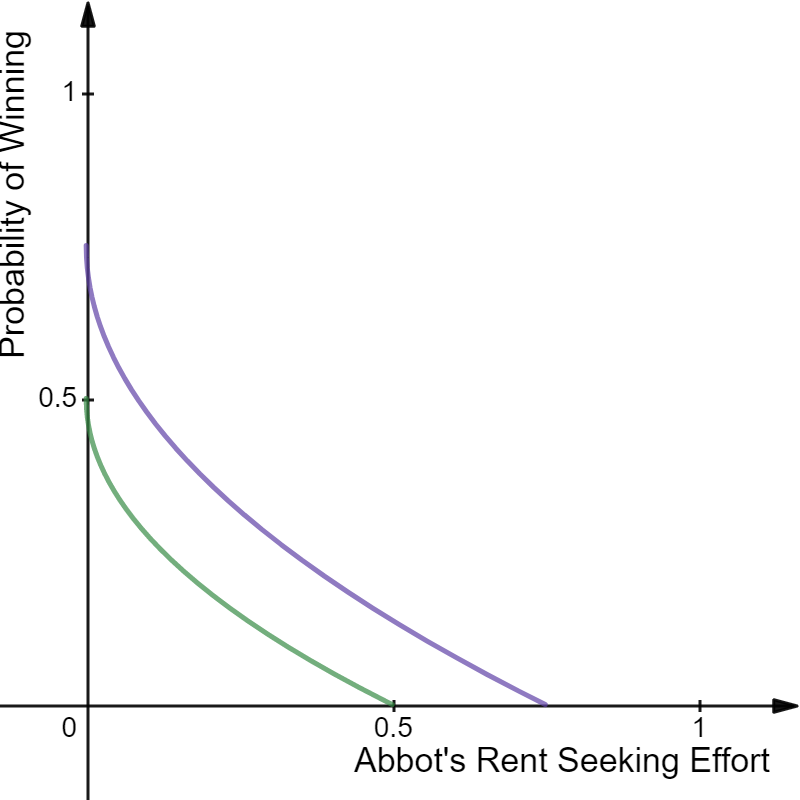
\includegraphics[width=0.6\linewidth]{probabilities.png}
    \caption{Kevin Rudd (Purple) and Julia Gillard's (Green) probabilities of winning given Tony Abbot's rent seeking effort.}
    \label{fig:probabilities}
\end{figure}
Substituting the specific values from the previous question verifies the claim that Labor should choose Rudd in favour of Gillard:
$$p_{g} = \frac{0.5 \times 0.1036}{0.1036 + 0.25} \approx 0.1464 \quad < \quad 0.3170 \approx \frac{0.75 \times 0.1830}{0.1830 \times 0.25} = p_{r}$$
\newpage
\vspace*{\fill}
\centering
Kevin 07 is also a significantly better downball player, so she never really stood a chance.
\begin{figure}[hb]
    \centering
    
\includegraphics[width=0.75\linewidth]{handball}
    \caption{Kev Shows Julia that he's the King of the Court.}
    \label{fig:handball}
\end{figure}
\vspace*{\fill}
\end{document}